\documentclass[conference]{IEEEtran}

\usepackage{amsmath,amssymb,bm}
\usepackage{graphicx}
\usepackage{float}
\usepackage{algorithm}
\usepackage{algpseudocode}
\usepackage{hyperref}
\usepackage{cite}

\title{Optical Initial Orbit Determination of the International Space Station Using Laplace's Method}

\author{Scott~Nguyen
	\thanks{Scott Nguyen is with the Department of Mechanical Engineering, University of New Mexico, Albuquerque, NM, USA (email: [scott.nguyen@unm.edu](mailto:scott.nguyen@unm.edu)).}}

\begin{document}
	
	\maketitle
	
	\begin{abstract}
		This paper presents an optical initial orbit determination (IOD) study of the International Space Station (ISS) using Laplace's method. Synthetic right ascension and declination measurements are generated from a ground-based optical sensor model incorporating Earth rotation and topocentric geometry. The resulting orbit solution is compared against truth data, and sensitivity to measurement noise is assessed through Monte Carlo analysis. Results highlight the limitations of classical batch IOD under noisy measurements and motivate sequential filtering approaches for autonomous navigation.
	\end{abstract}
	
	\begin{IEEEkeywords}
		Optical navigation, initial orbit determination, Laplace's method, space situational awareness, autonomous navigation.
	\end{IEEEkeywords}
	
	\section{Introduction}
	Optical navigation plays a critical role in space situational awareness and autonomous spacecraft operations. Classical initial orbit determination techniques, such as Laplace's method, enable orbit reconstruction using limited line-of-sight measurements but are highly sensitive to noise and modeling assumptions. This work applies Laplace's method to synthetic optical observations of the ISS to evaluate estimator performance and robustness.
	
	\section{Problem Setup}
	The ISS orbital elements at the initial epoch of 25 April 2025, 17:56 UTC are summarized in Table~\ref{tab:ISS_COEs}. These elements are converted to Earth-centered inertial (ECI) position and velocity vectors and propagated under a two-body Earth model.
	
	\begin{table}[H]
		\caption{Classical Orbital Elements of the ISS}
		\label{tab:ISS_COEs}
		\centering
		\begin{tabular}{ll}
			\hline
			Orbital Element & Value \
			\hline
			Epoch (UTC) & 25 April 2025 17:56 \
			Semi-major axis, $a$ & 6785.6 km \
			Eccentricity, $e$ & 0.00023 \
			Inclination, $i$ & 51.6367$^\circ$ \
			RAAN, $\Omega$ & 13.9687$^\circ$ \
			Argument of perigee, $\omega$ & 82.7408$^\circ$ \
			True anomaly, $\nu$ & 281.9577$^\circ$ \
			\hline
		\end{tabular}
	\end{table}
	
	The ground-based optical sensor is assumed to be located in Albuquerque, New Mexico, at latitude $35.0844^\circ$ and longitude $-106.6504^\circ$.
	
	\section{Optical Measurement Model}
	Line-of-sight (LOS) vectors are generated by transforming the ISS state into the topocentric horizon frame and computing azimuth and elevation angles. These measurements are converted to right ascension and declination in the ECI frame. Algorithm~\ref{alg:LOS} summarizes the LOS computation procedure.
	
	\begin{algorithm}[H]
		\caption{Line-of-Sight Measurement Computation}
		\label{alg:LOS}
		\begin{algorithmic}[1]
			\For{each observation time}
			\State Compute GMST and Earth rotation angle
			\State Transform ISS state to topocentric frame
			\State Compute LOS unit vector
			\State Extract azimuth, elevation, right ascension, and declination
			\EndFor
		\end{algorithmic}
	\end{algorithm}
	
	Figure~\ref{fig:ISS_trajectory} shows the propagated ISS trajectory relative to the sensor location, while Fig.~\ref{fig:Az_El} illustrates the resulting angular measurements.
	
	\begin{figure}[H]
		\centering
		
\includegraphics[width=0.9\columnwidth]{plots/fig_1.png}
		\caption{ISS trajectory relative to the ground-based sensor.}
		\label{fig:ISS_trajectory}
	\end{figure}
	
	\begin{figure}[H]
		\centering
		
\includegraphics[width=0.9\columnwidth]{plots/fig_2.png}
		\caption{Right ascension vs. declination and azimuth vs. elevation.}
		\label{fig:Az_El}
	\end{figure}
	
	\section{Initial Orbit Determination}
	Three closely spaced optical measurements are selected near maximum elevation. Laplace's method is applied to compute the satellite range by solving the resulting eighth-order polynomial. The physically meaningful root is selected based on expected orbital altitude.
	
	The estimated state is compared against the true propagated state, and percent errors are computed for position and velocity components.
	
	\section{Noise Sensitivity and Monte Carlo Analysis}
	Gaussian noise with a standard deviation of $0.01^\circ$ is added to azimuth and elevation measurements. The perturbed measurements are processed through the same IOD pipeline. Figure~\ref{fig:Histogram} presents the distribution of state errors over 1000 Monte Carlo trials.
	
	\begin{figure}[H]
		\centering
		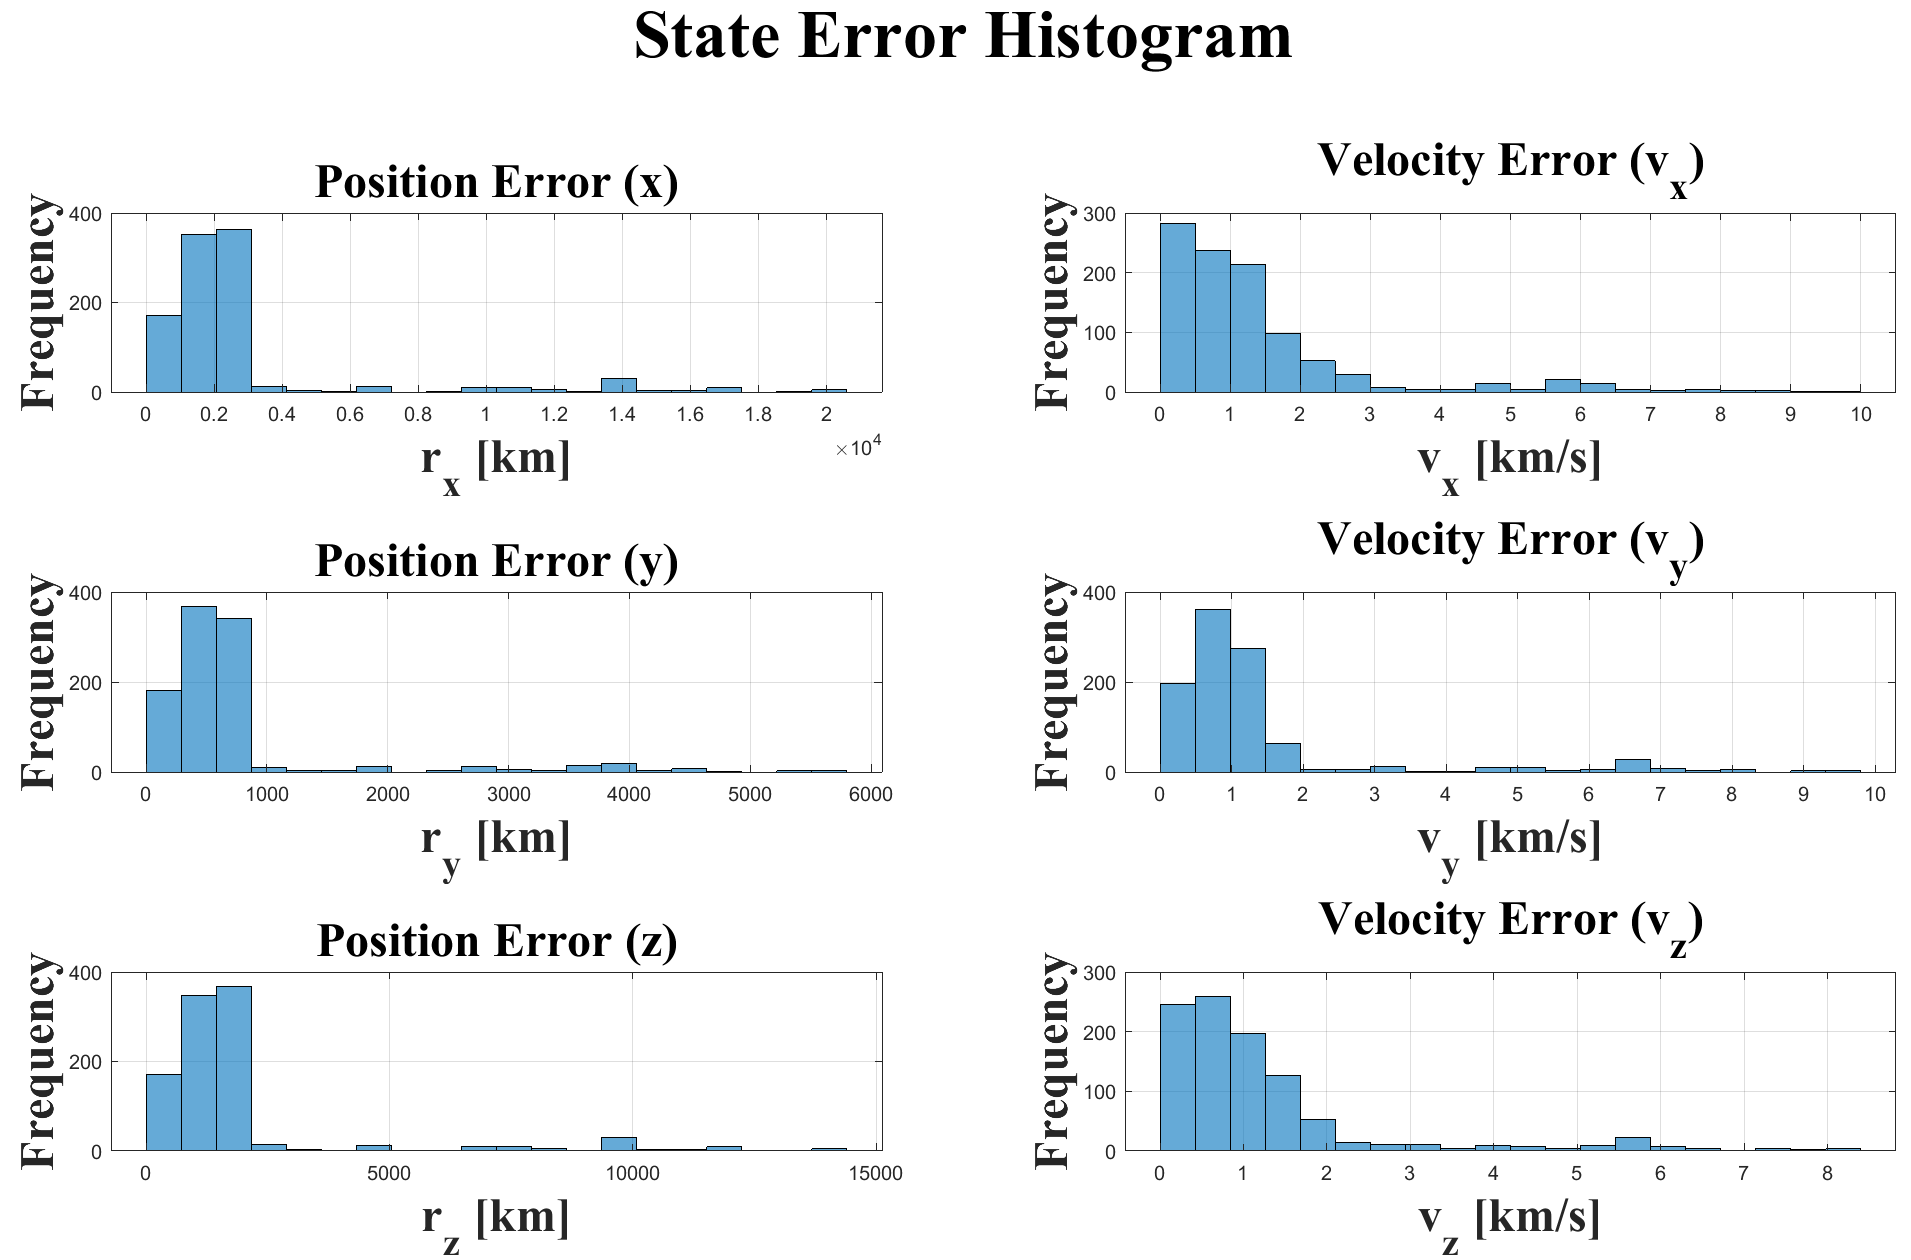
\includegraphics[width=0.9\columnwidth]{plots/fig_6.png}
		\caption{Histogram of state estimation errors from Monte Carlo analysis.}
		\label{fig:Histogram}
	\end{figure}
	
	Results indicate significant sensitivity to measurement noise, leading to large state dispersions over time when propagated.
	
	\section{Discussion}
	Results demonstrate that Laplace's method provides reasonable initial estimates under idealized conditions but exhibits significant sensitivity to measurement noise and simplified dynamics. Error growth over propagation underscores the limitations of batch IOD for autonomous navigation applications.
	
	\section{Conclusion}
	This study demonstrates an end-to-end optical navigation pipeline for initial orbit determination using Laplace's method. The results motivate the transition from batch IOD techniques to onboard filtering approaches for autonomous navigation applications.
	
	\section*{Acknowledgment}
	The author acknowledges coursework support from ME 594: Introduction to Space Situational Awareness at the University of New Mexico.
	
	\begin{thebibliography}{1}
		\bibitem{vallado}
		D. A. Vallado, \emph{Fundamentals of Astrodynamics and Applications}, 4th~ed. Microcosm Press, 2013.
	\end{thebibliography}
	
\end{document}
